\documentclass{beamer}
\usetheme{Rochester}
\usecolortheme{beaver}
\setbeamertemplate{caption}{\raggedright\insertcaption\par}
\setlength{\itemsep}{\fill}

\usepackage{graphicx}
\usepackage{multirow}
\usepackage{longtable}

\def\cvs{${[}$Id: slides.tex,v 1.19 2015/12/09 16:42:43 shettyr1 Exp ${]}$}

\beamertemplatenavigationsymbolsempty
\bibliographystyle{acm}

\newcommand{\slide}[1]{\scalebox{1.0}{\includegraphics[page=#1]{slides}}}
\newcommand{\mct}[1]{\multicolumn{2}{c|}{\bf#1}}
\newcommand{\mcCell}[1]{\multicolumn{1}{|c|}{#1}}
\newcommand{\bs}{\small\bf}
\newcommand{\red}[1]{\protect\begin{color}{red}#1\protect\end{color}}
\newcommand{\green}[1]{\protect\begin{color}{green}#1\protect\end{color}}
\begin{document}

%%-----------------------------------------------------------------------------

\title{Frame- and Segment-Level Features and Candidate Pool Evaluation for Video Caption Generation}
\subtitle{ACM Multimedia Grand Challenge Presentation}
\author[Rakshith Shetty and Jorma Laaksonen]{Rakshith Shetty and Jorma Laaksonen}
\institute{Department of Computer Science, \\Aalto University}
\date{\today}

\frame{\titlepage} 

%%\frame{\frametitle{Table of contents}\tableofcontents} 

%%-----------------------------------------------------------------------------
\section{Overview}
\begin{frame}{Our approach}
%\begin{itemize}
        %\item Standard Encoder--Decoder caption generation module.
        %\item Video featueres from two-different paradigms.
        %   \begin{itemize}
        %     \item Frame-level features for object and attributes
        %     \item Segment-level features for actions
        %   \end{itemize}
        %\item Train multiple caption generators with different feature combinations.
        %\item Ensemble using an evaluator network 
%\end{itemize} 
\begin{figure}[h]
    \centering
    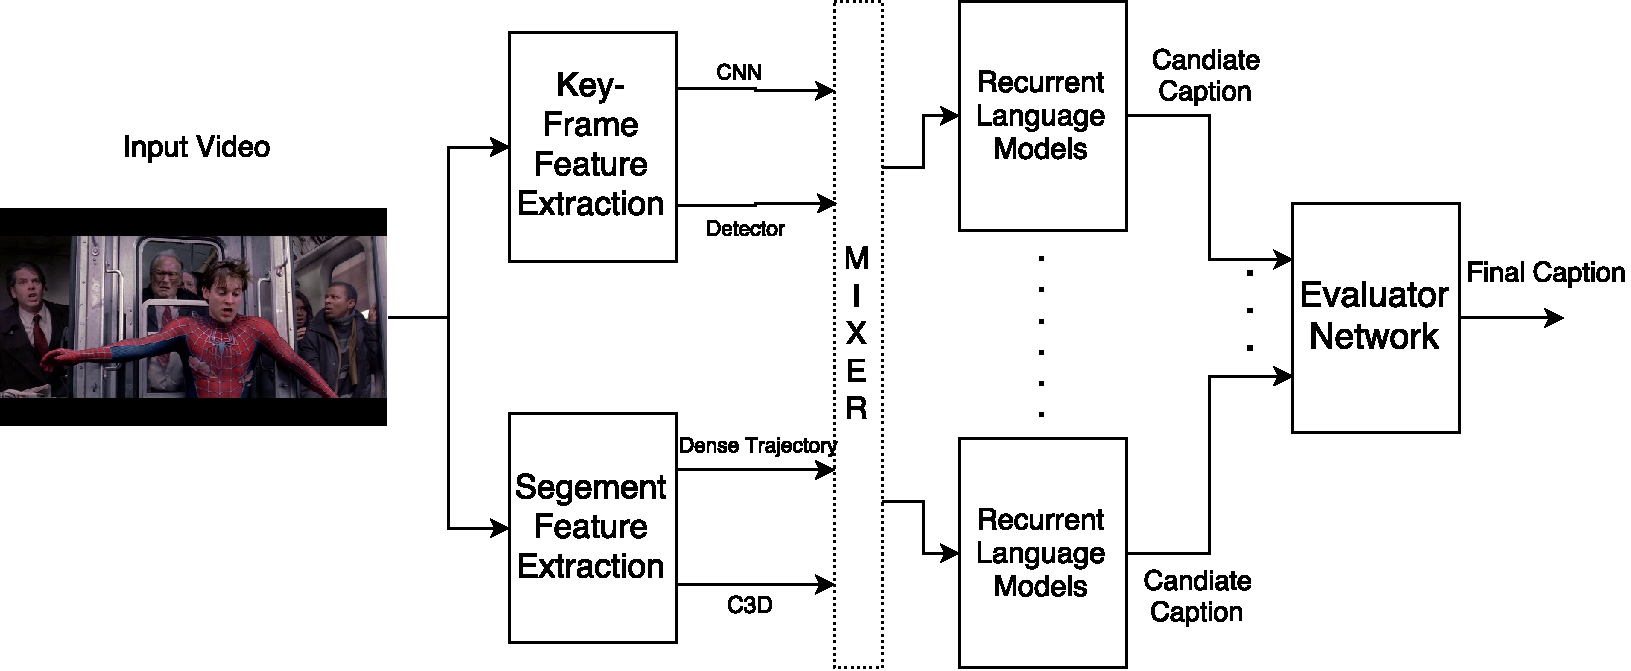
\includegraphics[width=1.0\textwidth]{images/MMGC_Overview.pdf}
\end{figure}
\end{frame}
%%-----------------------------------------------------------------------------
%\begin{frame}{Training and Generation}
%    \begin{itemize}
%        \item Pick a caption--image pair and maximize the probability assigned to caption 
%        \item Minimize the negative log likelihood 
%            \begin{align*}
%              \mathcal{NL}(w_0,\cdots, w_{L-1} | V) = -\sum_{t=0}^{L-1} \log(p(w_t|w_{t-1},V))
%            \end{align*}
%        \item Stochastic gradient descent using RMSProp 
%        \item Training limited to language model parameters 
%        \item Beamsearch is used in test mode to generate captions 
%    \end{itemize}
%\end{frame}
%%-----------------------------------------------------------------------------
%%=============================================================================
\section{Visual Features}
%%-----------------------------------------------------------------------------
\begin{frame}{Video Features}
    \centering
    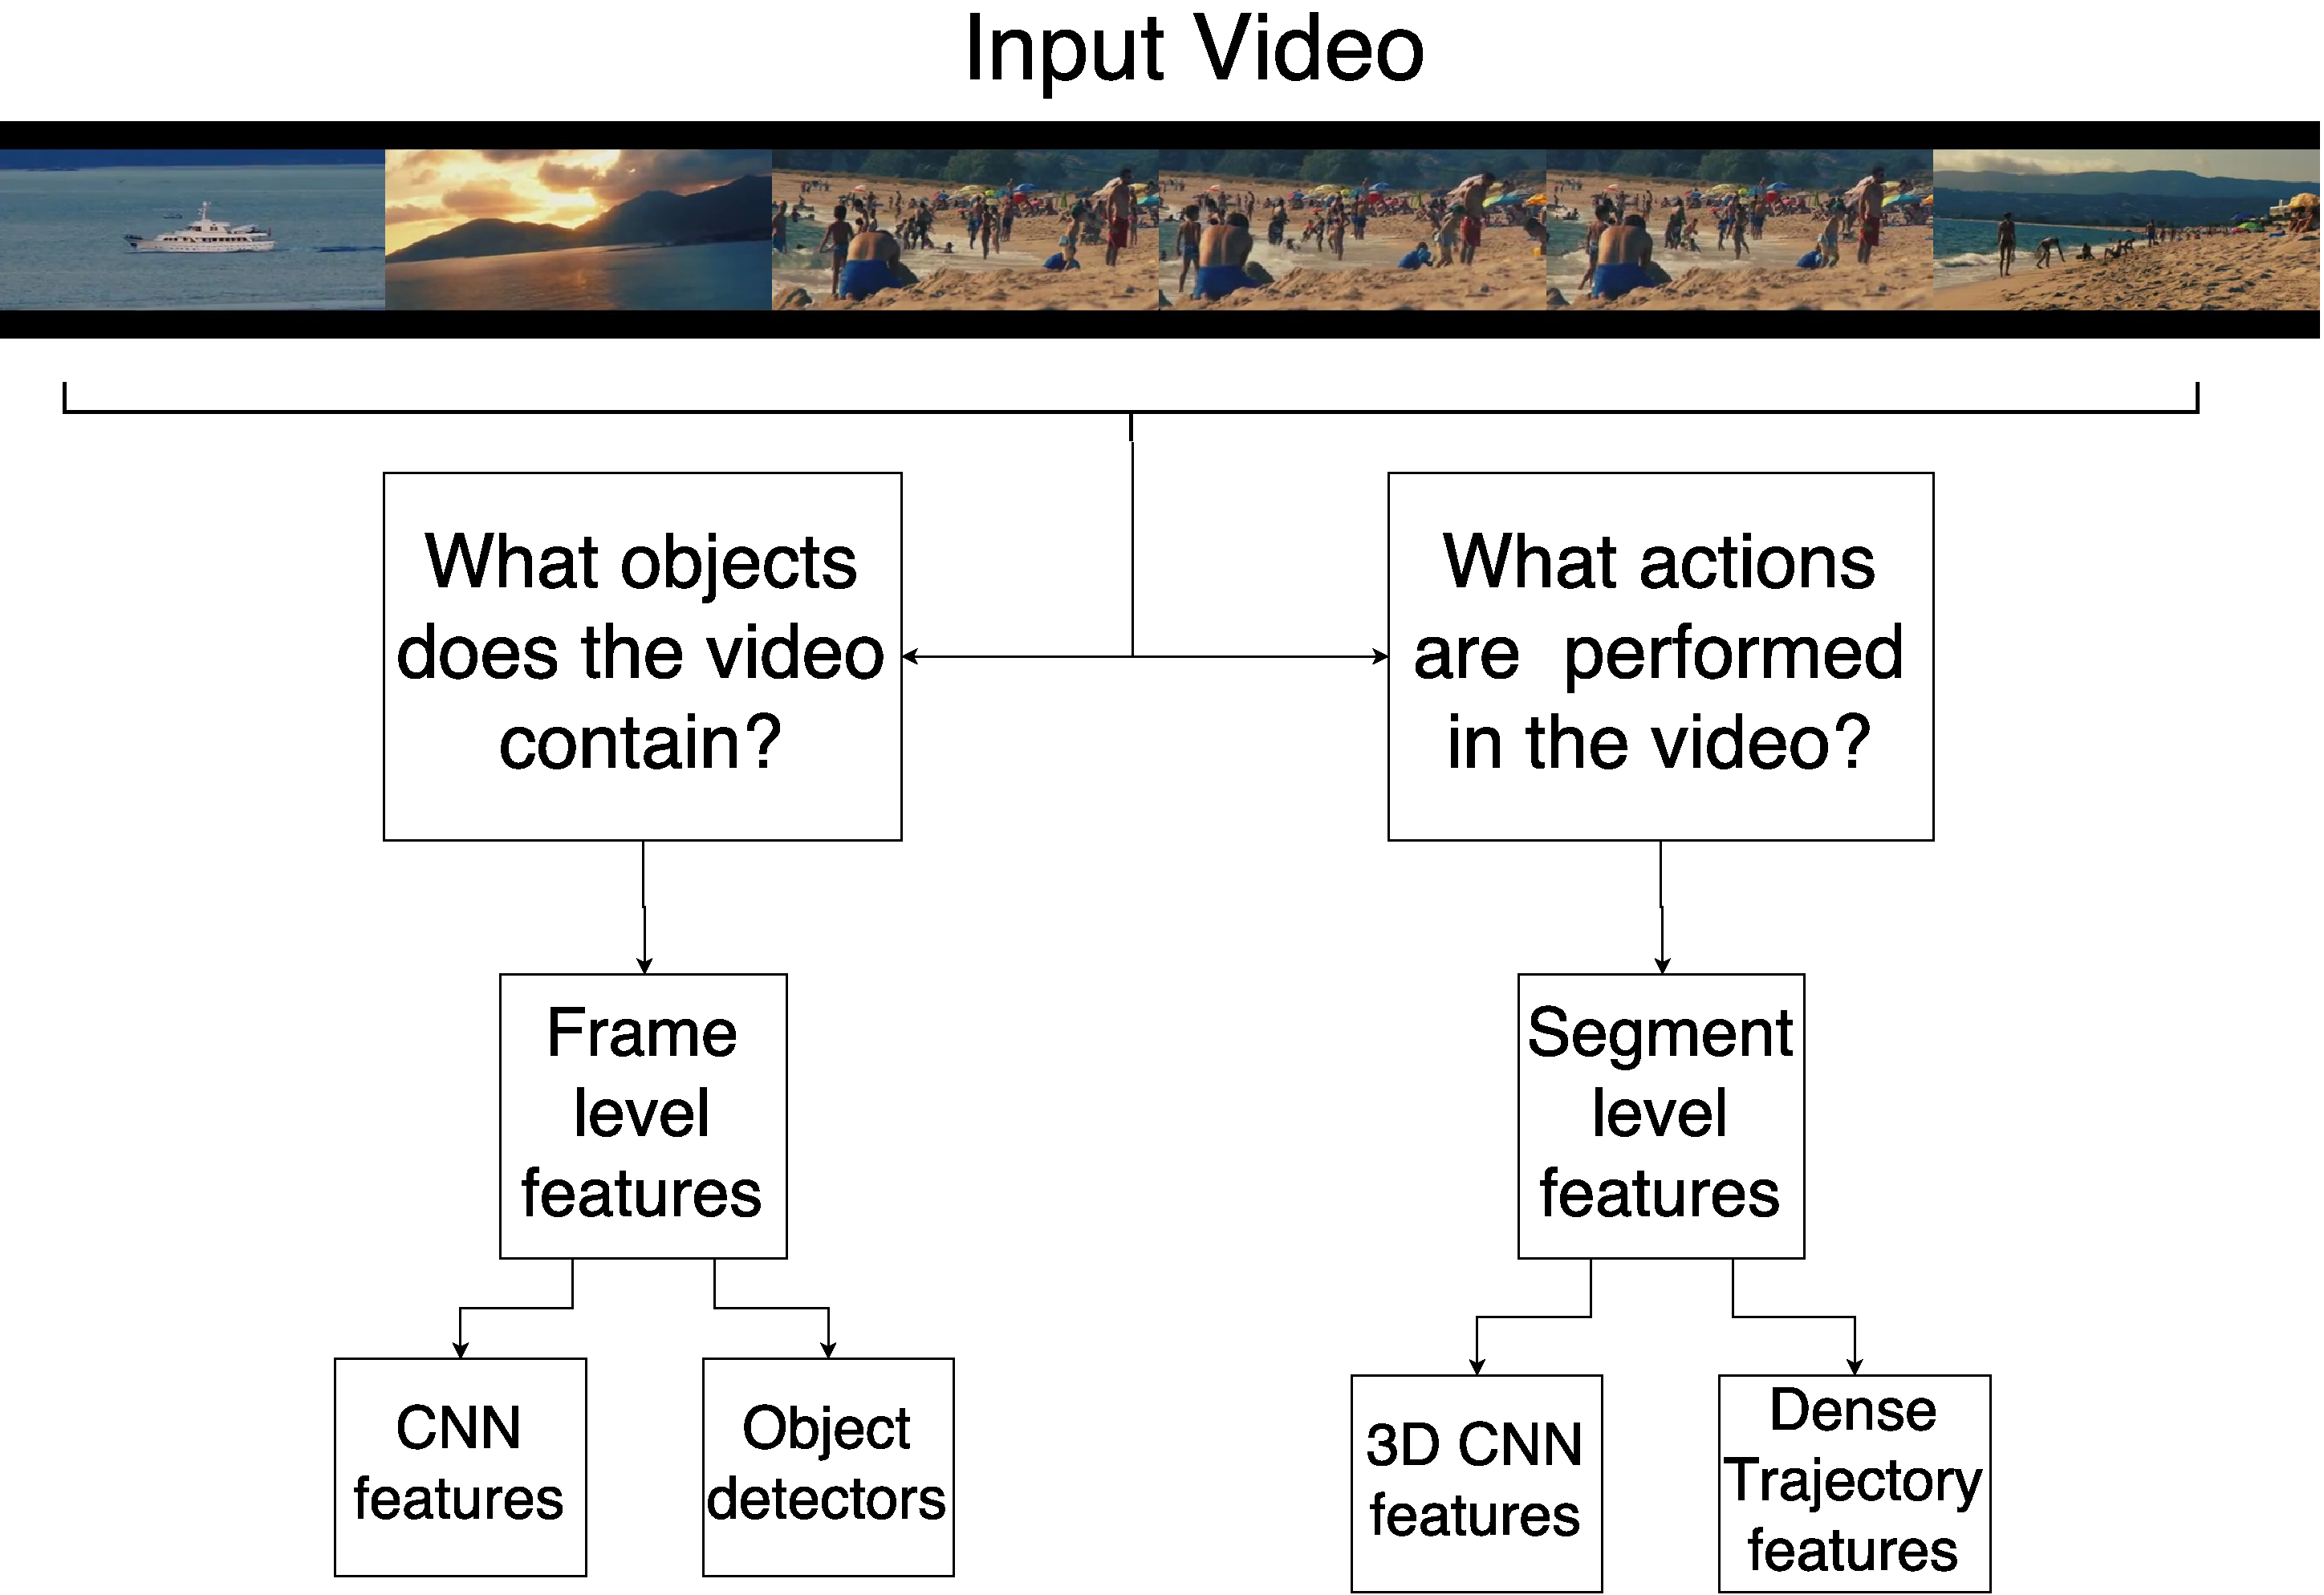
\includegraphics[width=1.0\textwidth]{images/VideoFeatures.pdf}
\end{frame}
%%-----------------------------------------------------------------------------
\begin{frame}{Language Model}
    \begin{figure}[h]
        \centering
        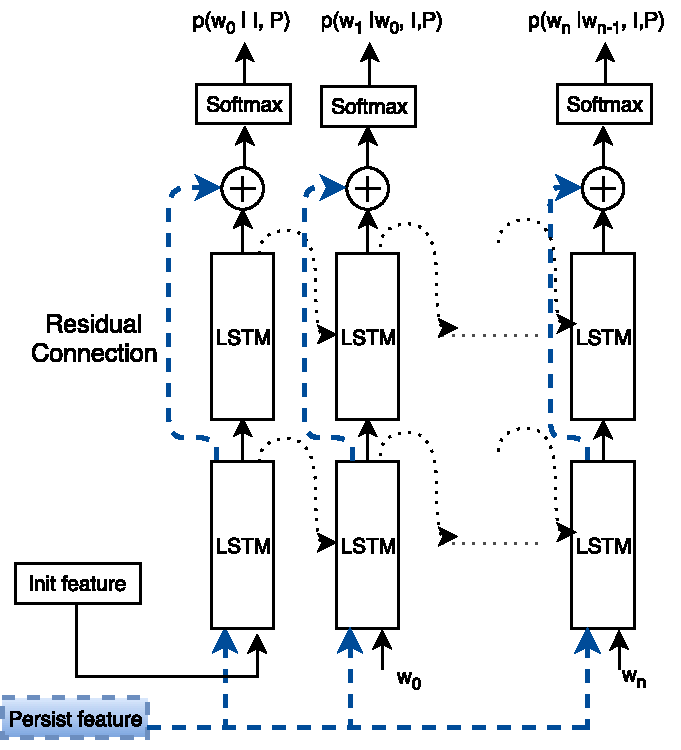
\includegraphics[width=0.5\textwidth]{images/MultilayerResidualLSTM.pdf}
    \end{figure}
    \begin{itemize}
        \item Use multiple layers of LSTM with \textbf{Residual} connections~\cite{He2015} 
        \item Two input channels -- \emph{init} and \emph{persist} 
    \end{itemize}
\end{frame}
%%-----------------------------------------------------------------------------
\section{Ensembling}
\begin{frame}{Why Ensembling?}
\begin{itemize}
        \item Dataset -- Various types of videos
        \item Features -- No single best feature
        \item Models -- Self-Evaluation can't be trusted
\end{itemize}
\underline{Example}
\begin{columns}       
    \column{0.4\linewidth}
    \begin{figure}[h]
        \centering
        \includegraphics[width=1.0\linewidth]{images/6774.png}
        \vfill
    \end{figure}
    \column{0.6\linewidth}
    \begin{figure}[thp]
      \begin{center}
      \centering
      \scalebox{0.9}{
      \begin{tabular}{|l|c|}
        \hline
        \textbf{\scriptsize\em Caption} &\textbf{\scriptsize\em Log-Prob}\\\hline
\textbf{\scriptsize\em \#1:} \scriptsize \red{a man is cooking}& \textbf{-3.89}  \\\hline
        \textbf{\scriptsize\em \#2:} \scriptsize \green{a man is eating food}& -5.20 \\\hline
        \textbf{\scriptsize\em \#3:} \scriptsize a man is cooking food & -6.64 \\\hline
      \end{tabular}
      }
        \vfill
      \end{center}
    \end{figure}
\end{columns}
\end{frame}
%%-----------------------------------------------------------------------------
\begin{frame}{Ensembling -- CNN evaluator}
\begin{columns}       
    \column{0.4\linewidth}
    \begin{figure}[h]
        \centering
        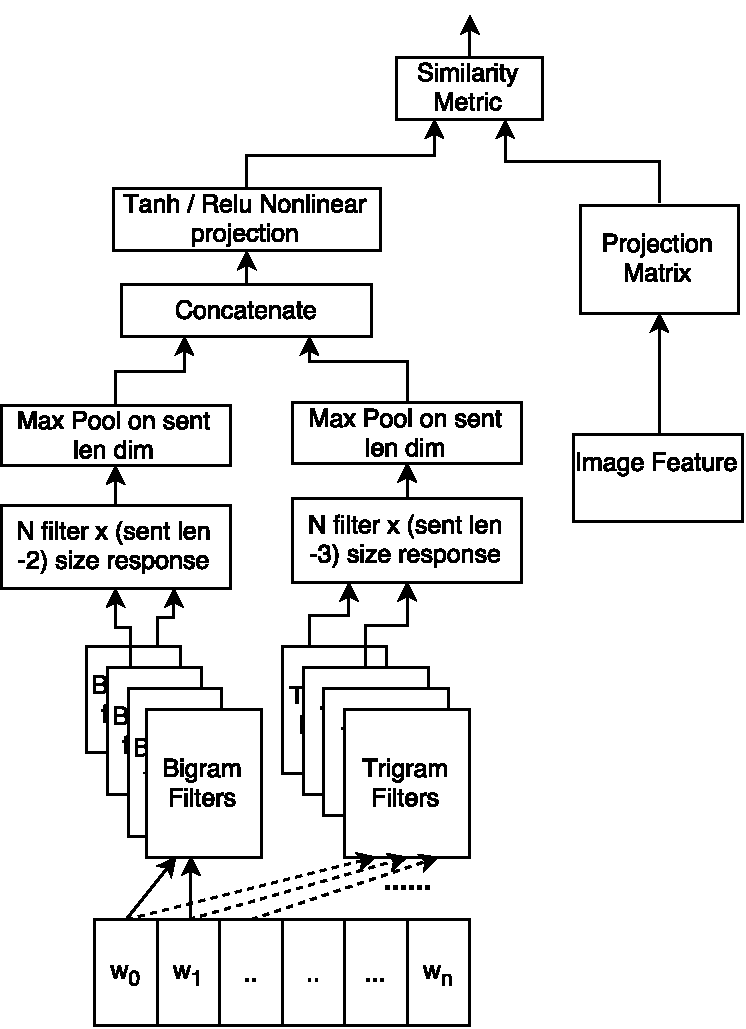
\includegraphics[width=1.0\textwidth]{images/CnnEval.pdf}
        \vfill
    \end{figure}
    \column{0.6\linewidth}
    \begin{itemize}
        \item Generative vs Discriminative 
        \item Train evaluator to compute similarity b/w visual input and caption 
           \begin{itemize}
               \item A CNN to encode the sentence 
               \item Visual feature is embedded to the same space 
               \item Cosine similarity b/w the two vectors 
           \end{itemize}
        \item Trained to assign highest score to correct caption--visual pair 
    \end{itemize}
\end{columns}
\end{frame}
%%-----------------------------------------------------------------------------
\begin{frame}{Does it work?}
\begin{columns}       
    \column{0.4\linewidth}
    \begin{figure}[h]
        \centering
        \includegraphics[width=1.0\linewidth]{images//6774.png}
        \vfill
    \end{figure}
    \column{0.6\linewidth}
    \begin{figure}[thp]
      \begin{center}
      \centering
      \scalebox{0.8}{
      \begin{tabular}{|l|c|c|}
        \hline
        \textbf{\scriptsize\em Caption} &\textbf{\scriptsize\em Log-Prob} &\textbf{\scriptsize\em CNN Score} \\\hline
\textbf{\scriptsize\em \#1:} \scriptsize a man is cooking& -3.89 & 0.86 \\\hline
        \textbf{\scriptsize\em \#2:} \scriptsize \green{a man is eating food}& -5.20 &\bf 0.89 \\\hline
        \textbf{\scriptsize\em \#3:} \scriptsize a man is cooking food & -6.64 & 0.87 \\\hline
      \end{tabular}
      }
        \vfill
      \end{center}
    \end{figure}
\end{columns}
\begin{table}[tbh]
  \centering
  \caption{Ensemble v/s single model on val set.}
  \scalebox{0.9}{
  \begin{tabular}{|l|c|c|c|c|c|}
    \hline
    Model &\bs BLEU-4 &\bs METEOR &\bs CIDEr &\bs ROUGE-L \\\hline\hline
    \small Best Single Model  & 0.409 & 0.268 & 0.433 & 0.598 \\
    \small CNN ensemble of 4 models & \bf0.411 & \bf0.277 & \bf0.464 & \bf0.596 \\\hline
  \end{tabular}
  }
  \label{tab:resVttFeat}
\end{table}
\end{frame}
%%-----------------------------------------------------------------------------
%%=============================================================================
\section{Results}
%%-----------------------------------------------------------------------------
%%-----------------------------------------------------------------------------
%\begin{frame}{Sample Validation Set Results}
%    \textbf{The Good}\\[2mm]
%    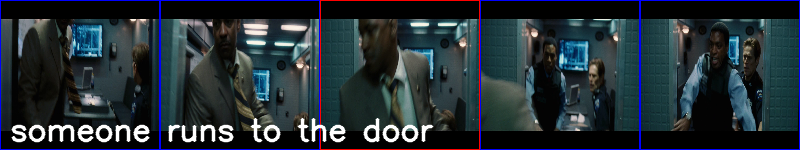
\includegraphics[width=0.5\textwidth]{images/230350439_genCap.png}\hspace*{0.01\textwidth} 
\includegraphics[width=0.5\textwidth]{images/110270280_genCapEdited.png}\\[2mm]
%    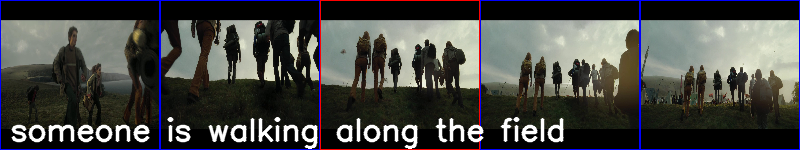
\includegraphics[width=0.5\textwidth]{images/110510033_genCap.png}\hspace*{0.01\textwidth} 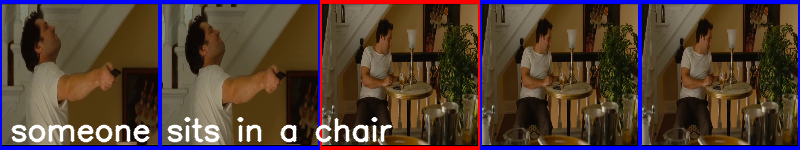
\includegraphics[width=0.5\textwidth]{images/140760125_genCap.png}\\[2mm]
%    \textbf{The Bad}\\[2mm]
%    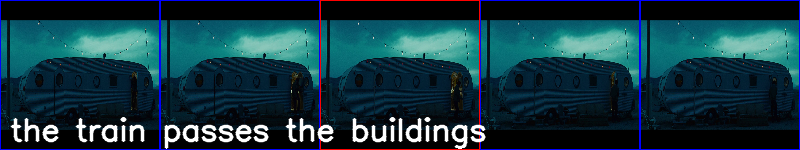
\includegraphics[width=0.5\textwidth]{images/110260059_genCap.png}\hspace*{0.01\textwidth} 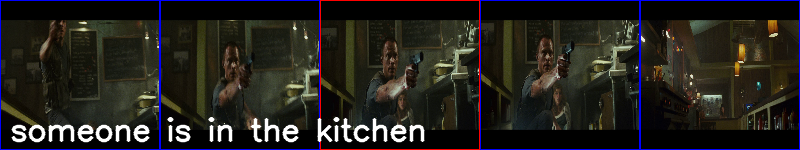
\includegraphics[width=0.5\textwidth]{images/110260532_genCap.png}\\[2mm]
%    \textbf{The Ugly}\\[2mm]
%    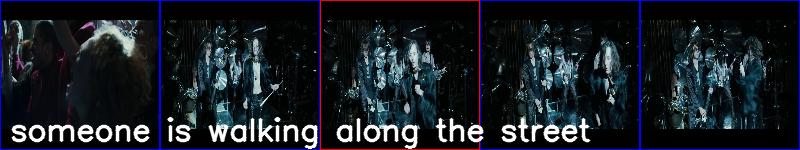
\includegraphics[width=0.5\textwidth]{images/110510496_genCap.png}\hspace*{0.01\textwidth} 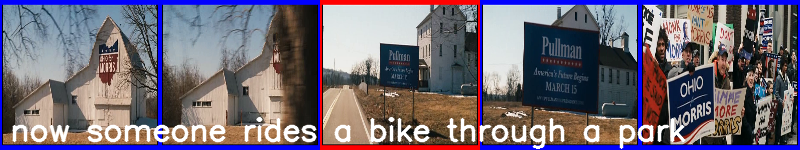
\includegraphics[width=0.5\textwidth]{images/140770020_genCap.png}\\
%\end{frame}
%%-----------------------------------------------------------------------------
\begin{frame}{MSR-VTT Experiments}
\begin{itemize}
    \item Frame-Level features were extracted from 1 frame per second 
    \item Three action recognition features: DT, IDT and C3D
    \item CNN ensemble \textbf{won} the MSR-VTT Challenge
\end{itemize}
\begin{columns}
    \column{.5\linewidth}
    \vspace{-5mm}
\begin{table}[tbh]
  \centering
  \scalebox{0.55}{
  \begin{tabular}{||c|c|c|c|c|}
    \hline\hline
    \bf Team  &\bs BLEU-4 &\bs METEOR &\bs CIDEr &\bs ROUGE-L \\\hline\hline
    v2t\_navigator &\bf0.408 &\bf0.282 & 0.448 &\bf0.609 \\
    \bf Aalto~(M6)     & 0.398 & 0.269 &0.457 & 0.598 \\
    VideoLAB       & 0.391 & 0.277 & 0.441 & 0.606 \\
    ruc-uva        & 0.387 & 0.269 &\bf0.459 & 0.587 \\
    Fudan-ILC      & 0.387 & 0.268 & 0.419 & 0.595 \\\hline
    \multicolumn{5}{||c|}{16 other teams with lower scores appear in the leaderboard}\\\hline
    \hline
  \end{tabular}}
\vspace{-2mm}
  \caption{Top 5 teams as per automatic evaluation metrics on test set.}
  \label{tab:resultsTestMet}
\end{table}
\column{.5\linewidth}
\begin{table}[tbh]
  \centering
  \scalebox{0.6}{
  \begin{tabular}{||c|c|c|c|}
    \hline\hline
    \bf Team  &\bs C1 &\bs C2 &\bs C3 \\\hline\hline
    \bf Aalto~(M6)     & \bf3.263 & 3.104 & \bf3.244\\
    v2t\_navigator & 3.261 & 3.091 & 3.154 \\
    VideoLAB       & 3.237 & \bf3.109 & 3.143 \\
    Fudan-ILC      & 3.185 & 2.999 & 2.979 \\
    ruc-uva        & 3.225 & 2.997 & 2.933 \\\hline
    \multicolumn{4}{||c|}{\parbox[c][][c]{8cm}{\smallskip\centering 16 other teams appear in the leaderboard\smallskip}}\\\hline
    \hline
  \end{tabular}
  }
\vspace{-2mm}
  \caption{Top 5 teams as per human evaluation.}
  \label{tab:resultsTestHum}
\end{table}
\end{columns}
\end{frame}
%%=============================================================================
\section{Conclusions}
%%-----------------------------------------------------------------------------
%\begin{frame}{Next.....}
%\tableofcontents[currentsection] 
%\end{frame}
%%-----------------------------------------------------------------------------
\begin{frame}{Conclusions}
\begin{itemize}
    \item Ensemble approach paid off! 
       \begin{itemize}
           \item Improved performance and caption diversity
           \item Different types of video features compliment each other well 
       \end{itemize}
    \item The language model extensions were useful. 
       \begin{itemize}
           \item The \emph{persist} input channel greatly improved performance
           \item The residual connections achieve lower training cost, and convergence time
       \end{itemize}
    \item Performance varies a lot across video categories 
    \item Our model performed the best according to human judgments  
\end{itemize}
\end{frame}
%%-----------------------------------------------------------------------------
\begin{frame}{}
\begin{center}
    \Large Thank You for Listening\\[6mm]
    \Large Any Questions? 
\end{center}
\end{frame}
%%-----------------------------------------------------------------------------
\begin{frame}{Sample Captions Video}
\begin{figure}[thp]
  \begin{center}
  \centering
  \tabcolsep=0.10cm
  \scalebox{0.7}{
          \begin{tabular}{|l|l|l|}
    \hline
    \mcCell{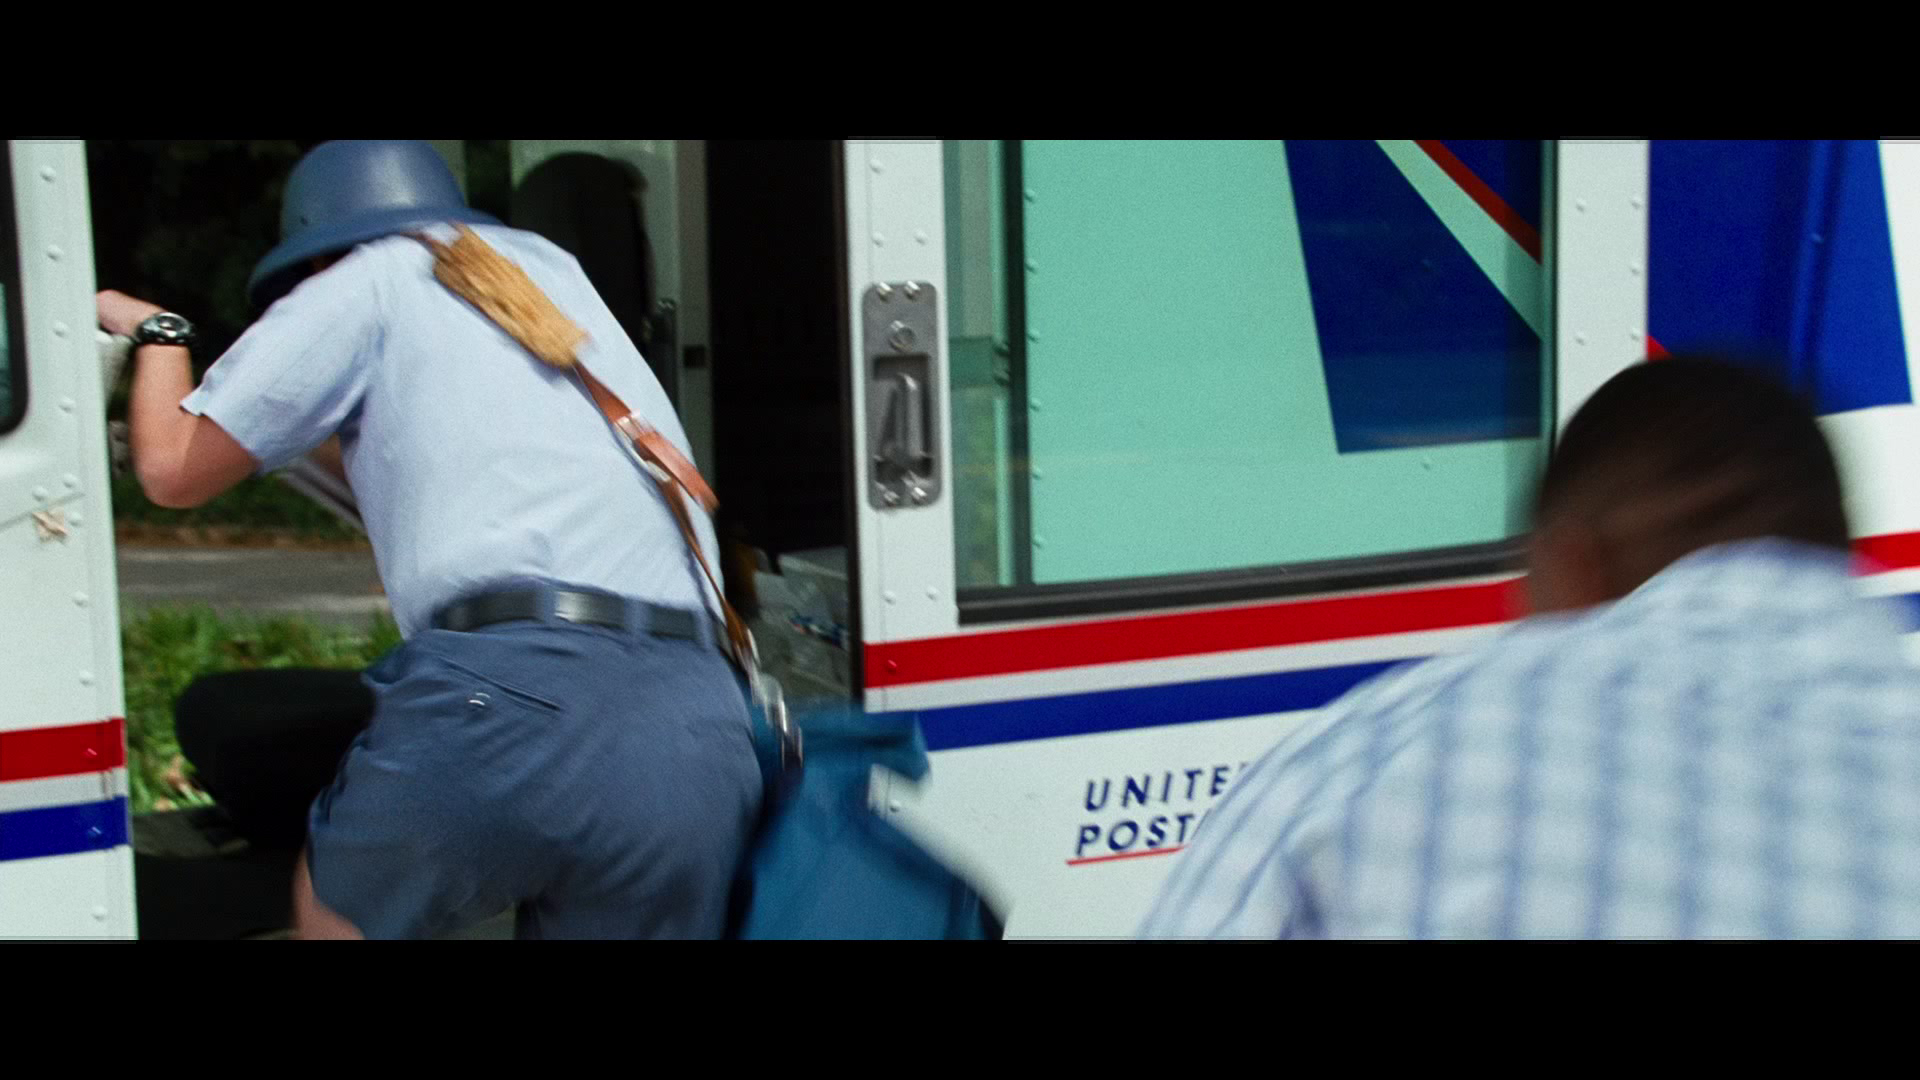
\includegraphics[width=0.25\linewidth]{images/LsmdcVid0.png}} &
    \mcCell{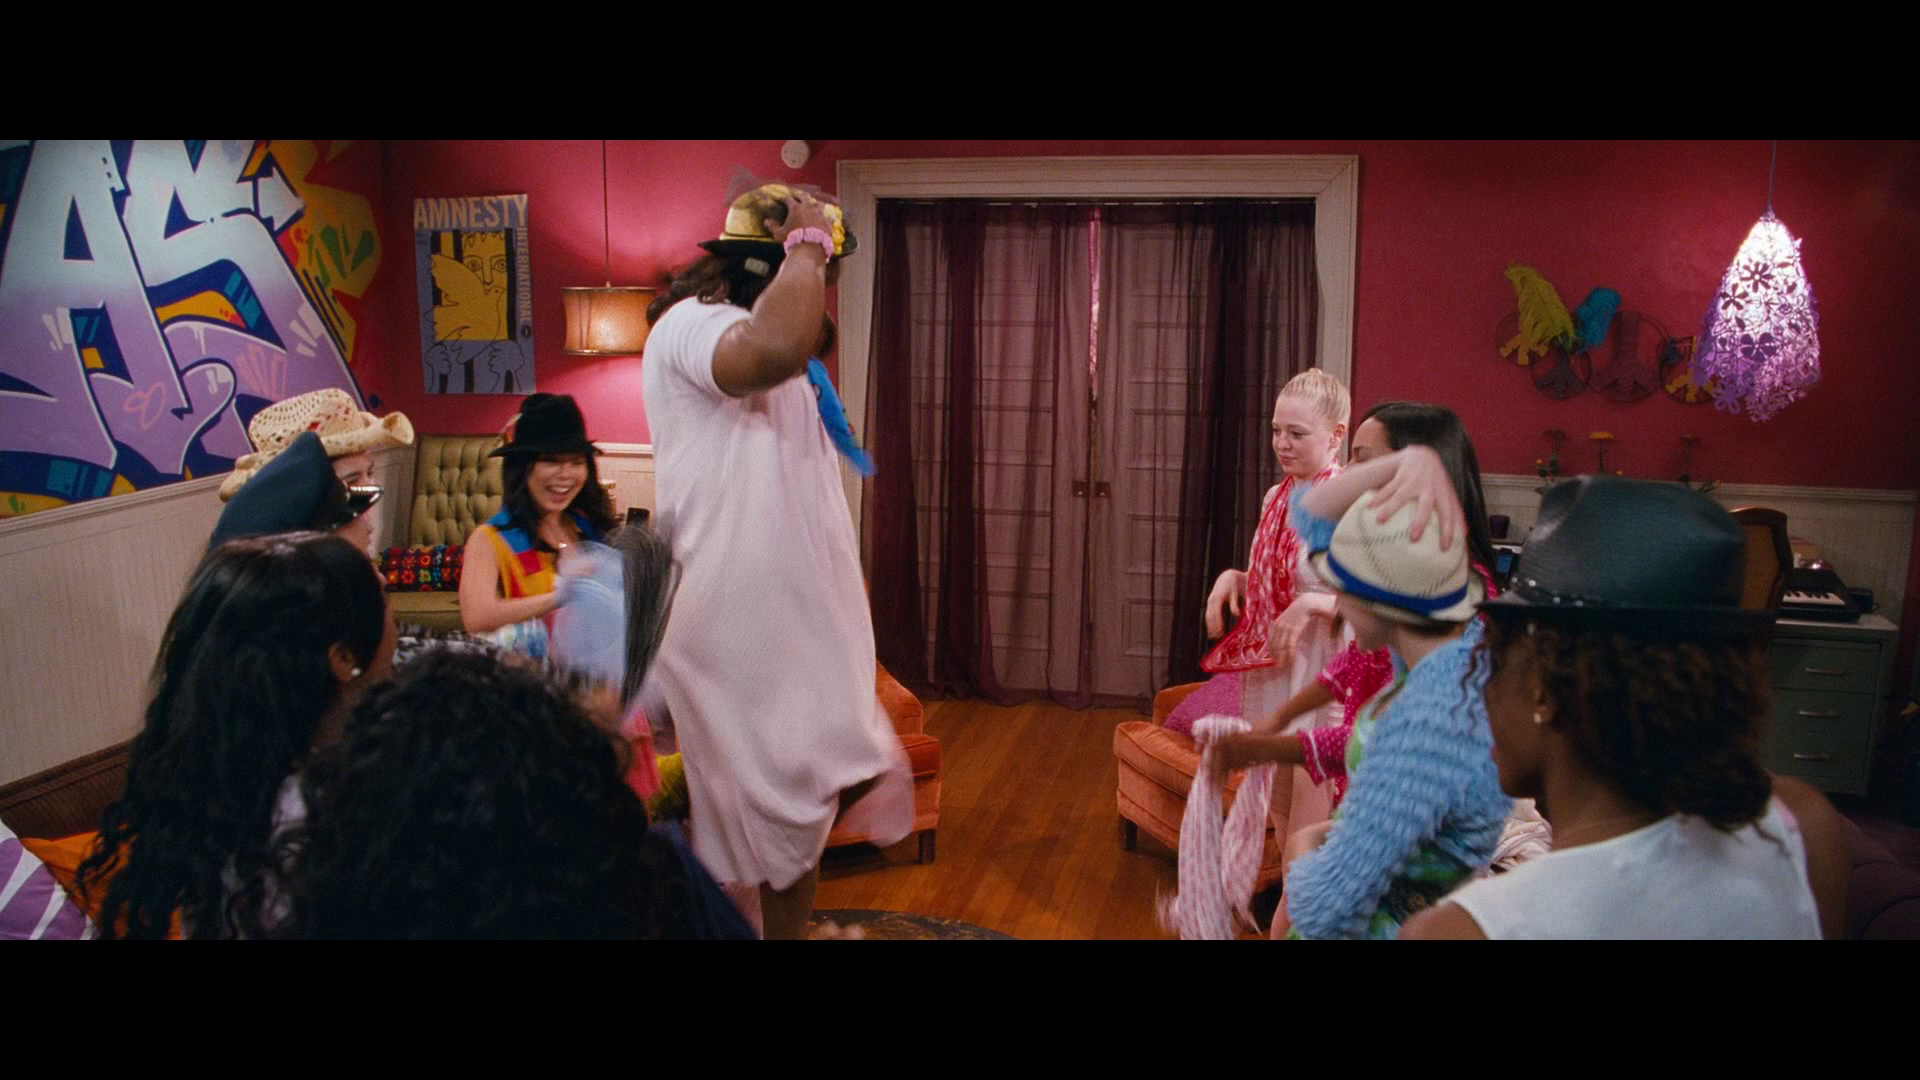
\includegraphics[width=0.25\linewidth]{images/LsmdcVid1.png}} &
    \mcCell{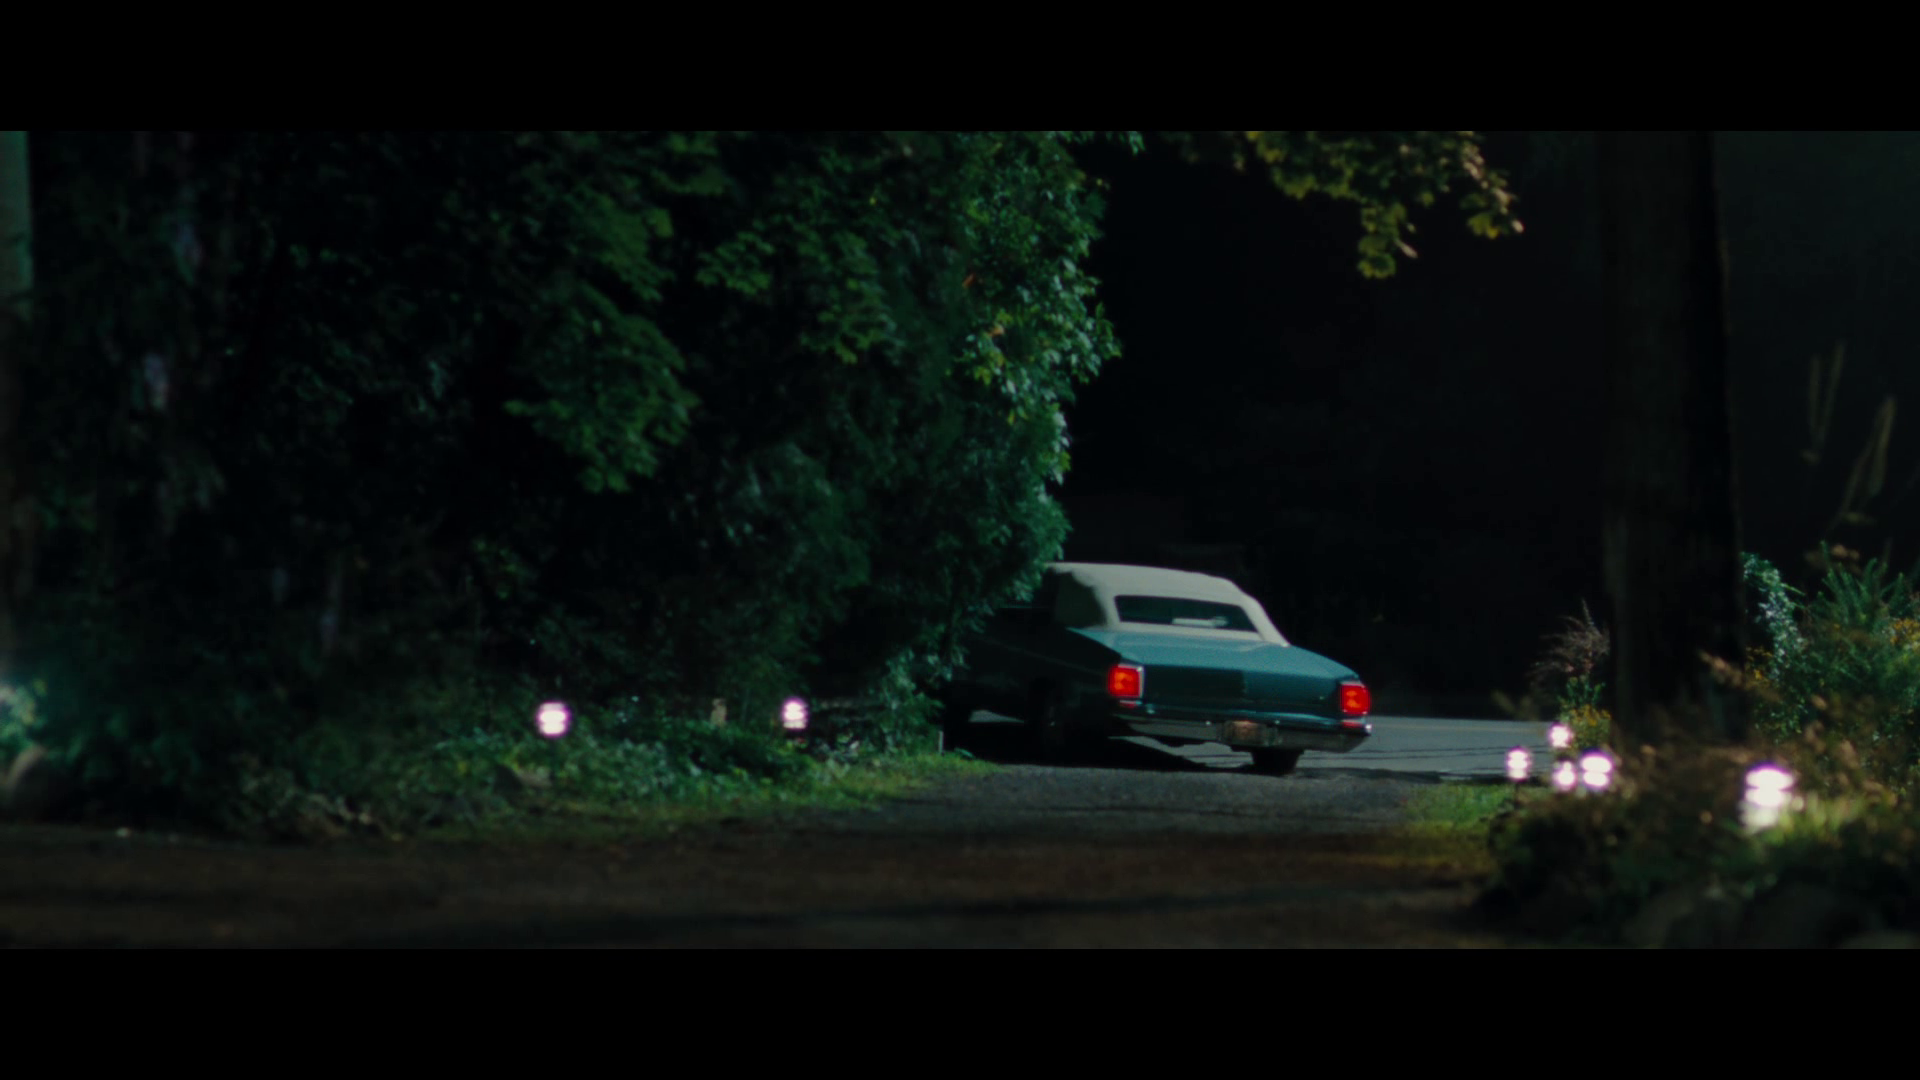
\includegraphics[width=0.25\linewidth]{images/LsmdcVid2.png}}
    \\\hline
    \textbf{\scriptsize\em L6:} \scriptsize someone runs up to the car&
    \textbf{\scriptsize\em L6:} \scriptsize someone is dancing with her&
    \textbf{\scriptsize\em L6:} \scriptsize someone looks up at the house\\\hline\\\hline
    \mcCell{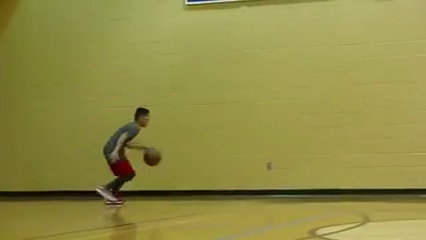
\includegraphics[width=0.25\linewidth]{images/9150.png}} &
    \mcCell{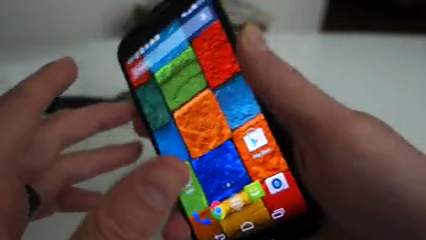
\includegraphics[width=0.25\linewidth]{images/9799.png}} &
    \mcCell{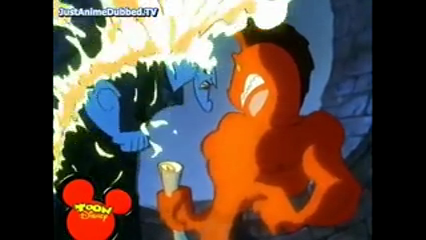
\includegraphics[width=0.25\linewidth]{images/7997.png}} \\\hline
    \textbf{\scriptsize\em M6:} \scriptsize a man is running in a gym &
    \textbf{\scriptsize\em M6:} \scriptsize a person is playing with a rubix cube &
    \textbf{\scriptsize\em M6:} \scriptsize cartoon characters are interacting\\
    \textbf{\scriptsize\em M2:} \scriptsize a man is running&
    \textbf{\scriptsize\em M2:} \scriptsize a man is holding a phone&
    \textbf{\scriptsize\em M2:} \scriptsize a person is playing a video game\\
    \textbf{\scriptsize\em M5:} \scriptsize a man is playing basketball&
    \textbf{\scriptsize\em M5:} \scriptsize a person is playing with a rubix cube &
    \textbf{\scriptsize\em M5:} \scriptsize a group of people are talking\\
    \hline
  \end{tabular}
  }
  \end{center}
  \label{fig:VttcapSamps}
\end{figure}
\end{frame}
%%-----------------------------------------------------------------------------
\begin{frame}{Qualitative Analysis}
\vspace{-5mm}
\begin{columns}
  \column{.5\linewidth}
  \begin{figure}[t]
    \centering
    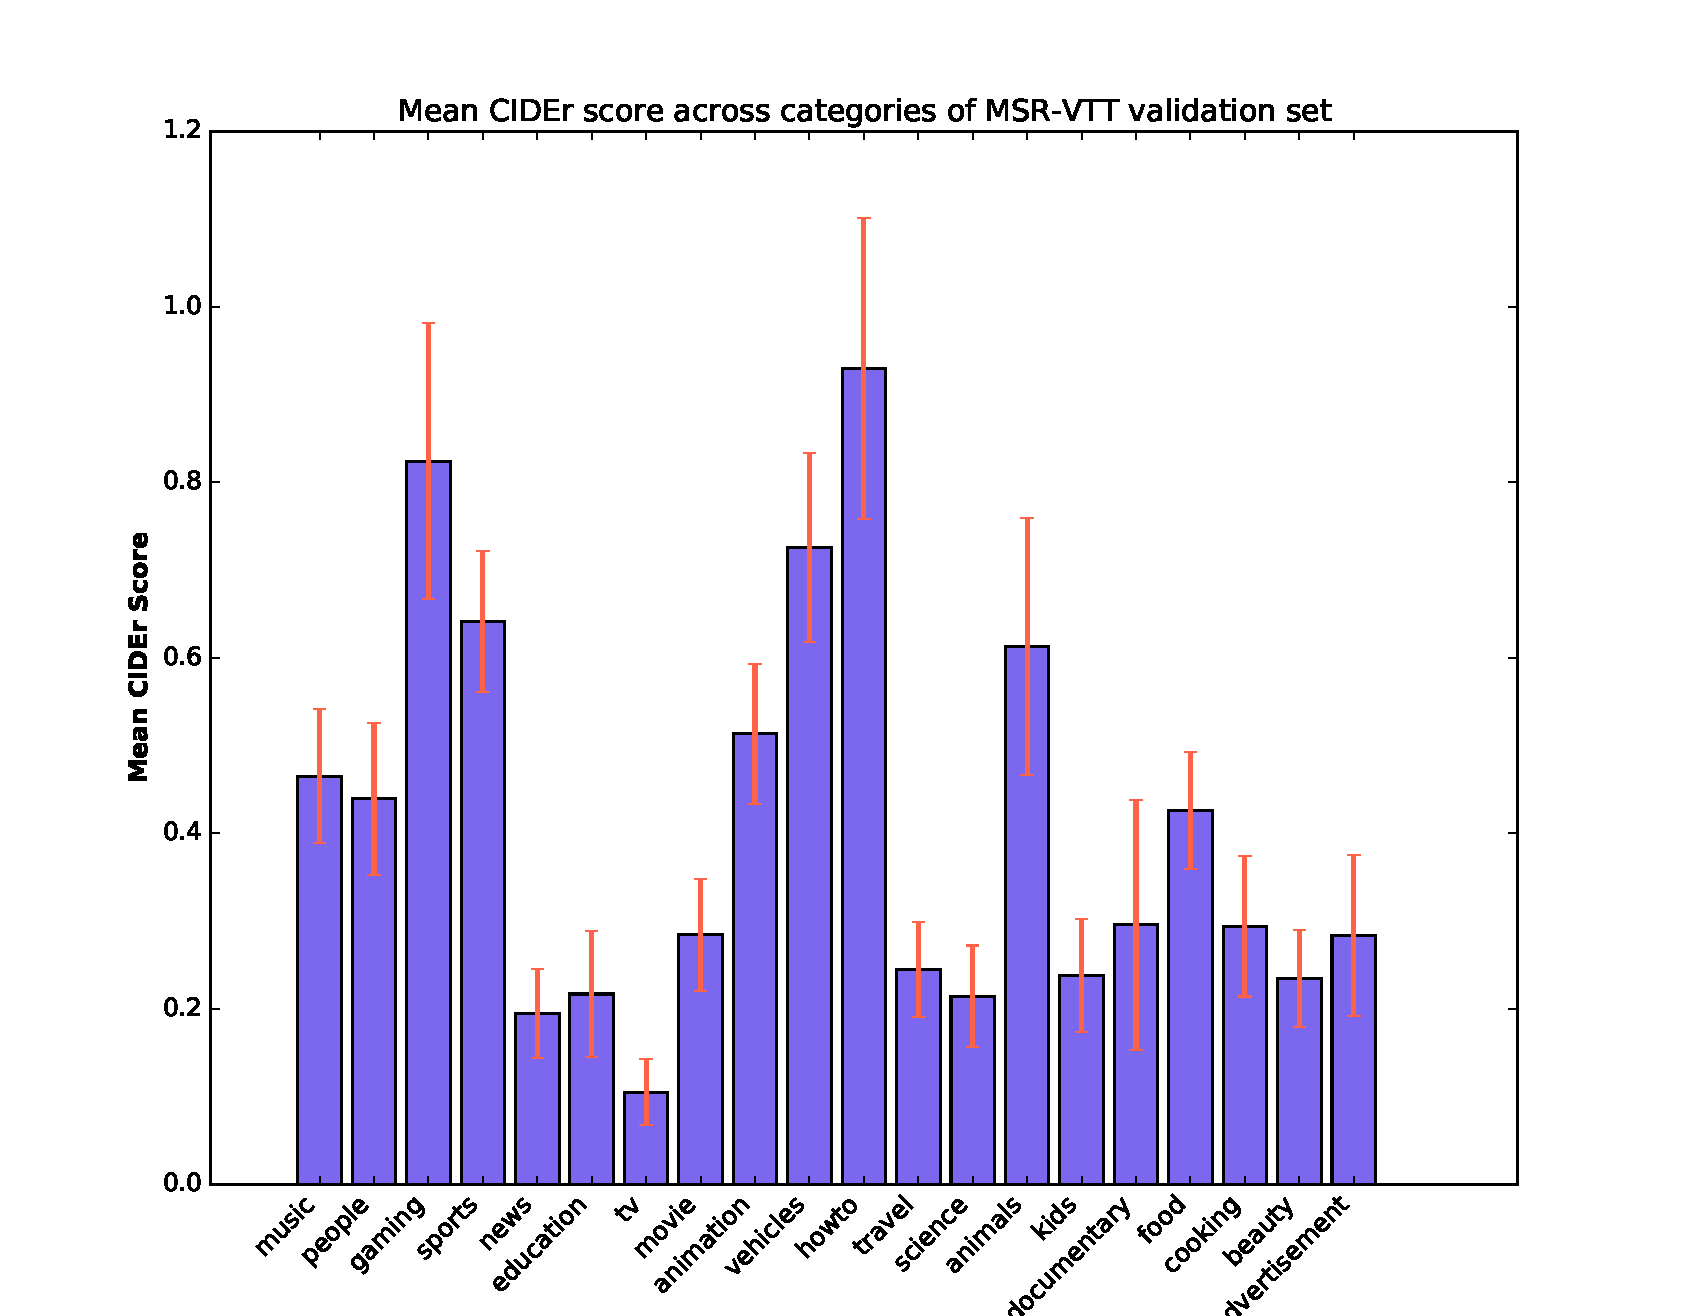
\includegraphics[trim={2cm 0 2cm 0},clip,width=0.8\linewidth]{images/VTTCiderCateg.pdf}
    \vspace{-5mm}
    \caption{Performance by video category}%
  \end{figure}
  \column{.5\linewidth}
  \begin{figure}[t]
    \centering
    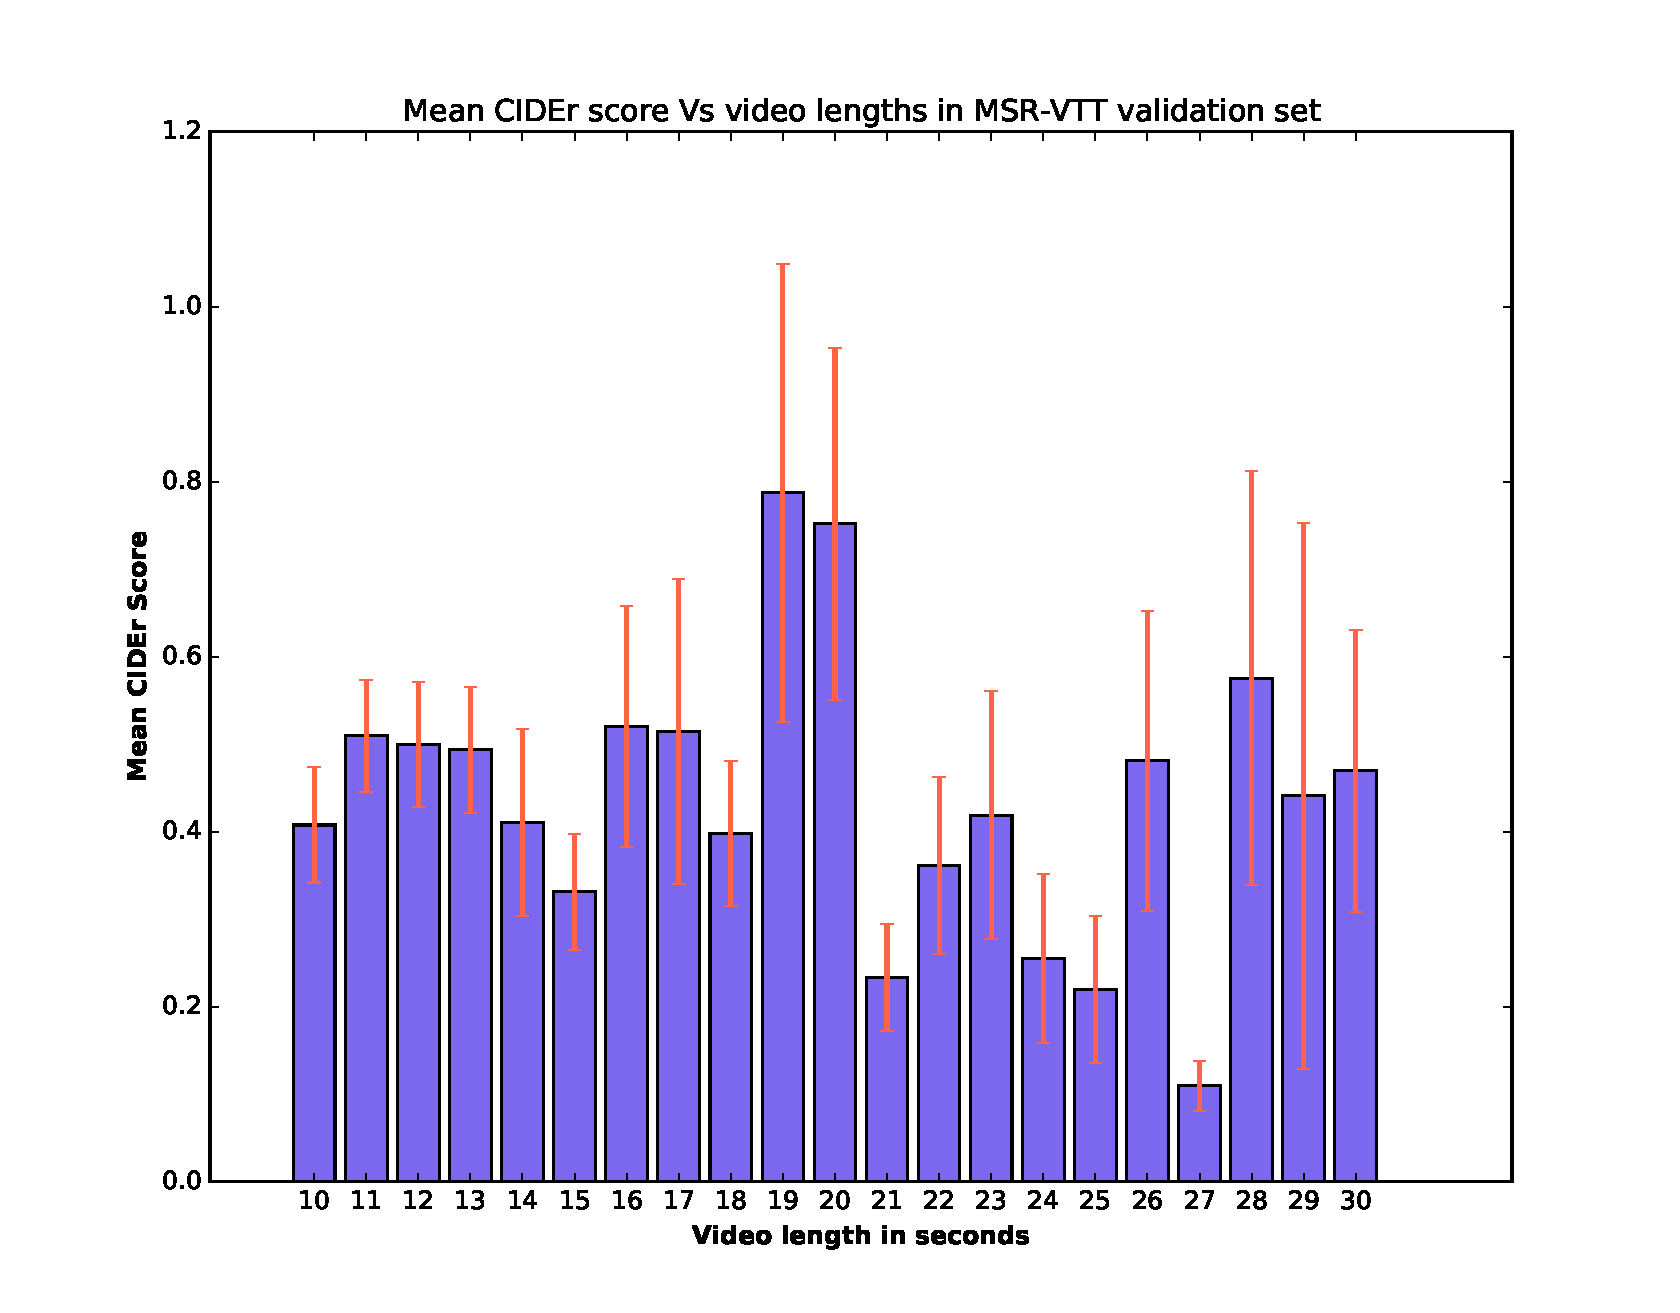
\includegraphics[trim={2cm 0 2cm 0},clip, width=0.8\linewidth]{images/VTTCiderLengths.pdf}
    \vspace{-5mm}
    \caption{Performance by video length}
    \label{fig:VttLenPerf}
  \end{figure}
\end{columns}
\begin{itemize}
    \item Video category has a huge impact
       \begin{itemize}
               \item \emph{How to}, \emph{video games} perform best 
               \item \emph{News}, \emph{tv} perform worst 
       \end{itemize}
    \item Surprisingly, length doesn't seem effect much (in-conclusive) 
\end{itemize}
\end{frame}
\begin{frame}[allowframebreaks]
        \frametitle{References}
        \bibliography{bib_thesis_used_only}
\end{frame}
%%-----------------------------------------------------------------------------
\end{document}
